\section{Теоретические основы типографики и верстки}

\subsection{История развития}

Современная наука указывает на то, что впервые формы для набора текста из фаянса были применены в Китае почти тысячу лет назад (1040 г.) слугой императора Би Шэном. И хоть использующийся для этого материал был недолговечен, вплоть до появления его в XIII веке в Корее подобной технологией никто не пользовался. С середины XV столетия типографика появилась в Европе, здесь и начался ее бурный расцвет, чему способствовала простота и небольшое количество букв в латинском шрифте, в отличие от китайских иероглифов\cite{typo_history}.

Первопроходцем европейской типографики считают немецкого ювелира и изобретателя Иоана Гутенберга. Именно он в 1440 году создал наборную форму из свинцовых букв и печатный станок. С их помощью можно было не только быстро и точно набрать нужный текст и отпечатать страницу, но и многократно использовать металлические символы. Первым шрифтом был выбран готический, так как он наиболее соответствовал рукописному тексту тех времен и содержал почти 300 знаков.

Важные события развития типографики:

\begin{itemize*}
	\item 1444--1446 гг. некий Прокопий Вальдфогель (подозревают, что это сам Гутенберг) заключает сделки с разными лицами по продаже технологии «искусственного письма».
	\item 1468 г. --- первая книга в Чехии.
	\item 1494 г. --- итальянский типограф Альд Мануций издал книгу с образцами шрифтов, которые уже лишь отдаленно напоминали рукописное письмо.
	\item 1517 г. --- первая книга на белорусском языке.
	\item 1563 г. --- первая крупная типография в Москве, во главе с Иваном Федоровым, который искусно проработал не только полууставной шрифт на основе рукописного письма, но и красочное оформление, поражающее мельчайшими деталями.
	\item 1580--1581 --- отпечатаны 1500 экземпляров библии в Острожской типографии.
\end{itemize*}

Со временем типографы начали осознавать важность удобочитаемости шрифта и начали изобретать формы, известные нам и сегодня:  Garamond, Century Schoolbook, Minion, Palatino, их создателем был Николас Йенсен. Дальнейшему развитию типографики характерно строгое соблюдение выключки, интерлиньяжа, появление абзацев\cite{about_font}.

Серьезную попытку по созданию научной основы этого искусства сделал француз Пьер Фурнье. Он издал в 1773 году «Типографическое руководство», в котором разработал систему определения кегля шрифта. Для его измерения он предложил использовать пики (picas) и пункты (points), а Франсуа Дидо приравнял 72 пункта к одному дюйму, подобная система используется до сих пор\cite{gordon_aboutletters}.

В 1750--1770 гг. англичанин Джон Баскервилл, отказавшись от книжного орнамента, сделал акцент на оформлении шрифта и создал шрифты так называемого переходного стиля, к которым относятся Baskerville, Gaslon, Bookman и всем известный Time New Roman. Особенностью их форм является сочетание строгой классики и особой элегантности, которую придают ему засечки.

Формат печатного листа изменялся крайне часто. В начале развития печати, каждый печатный мастер выбирал тот формат, который ему был удобен для конкретной книги. В книге Яна Чихольда <<Облик книги>>\cite{tschichold_image} собраны наиболее используемые размеры листа (рисунок~\ref{fig:formats}) за все время существования печати. На сегодняшний день в официальных документах РФ (в том числе и формальных отчетах) используется размер из международного стандарта ISO 216 --- A4 (I на рисунке)\cite{GOST732}, в США используется американский формат ANSI --- Letter ($\approx 1:1,3$)

\begin{figure}[H]
	\centering
	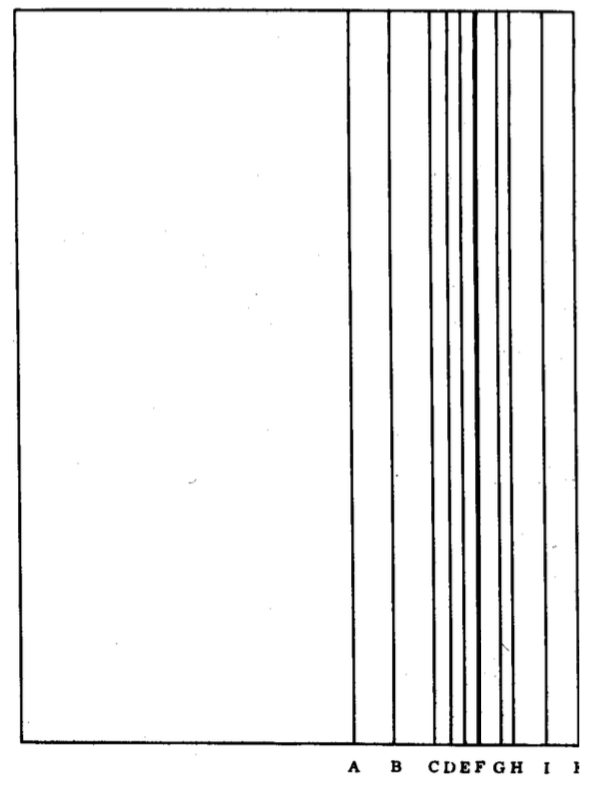
\includegraphics[width=0.55\textwidth]{pics/formats.png}
	\caption{Сравнительная ширина различных листов.\\
		A --- $1:2,236\ (1:\sqrt{5})$;
		B --- $1:2\ (1:\sqrt{4})$;
		C --- $5/9$;
		D --- $1:1,732\ (1:\sqrt{3})$;
		E --- $3:5$;
		F --- $1:1,618\ (21:34)$ (золотое сечение);
		G --- $1:1,538$;
		H --- $2:3$;
		I --- $1:1,414\ (1:\sqrt{2})$;
		K --- $3:4$
	}
	\label{fig:formats}
\end{figure}

\subsection{Общий вид печатного листа}

Поля страницы определяются форматом печатного листа, выбранным шрифтом, видом и назначением книги или документа. Как правило, поля для книжного разворота выбираются, как показано на рисунке~\ref{fig:margins}.

\begin{figure}[H]
	\centering
	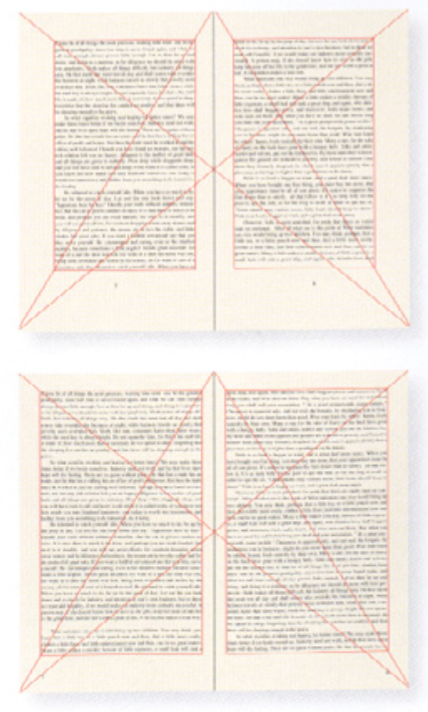
\includegraphics[width=0.55\textwidth]{pics/margins.png}
	\caption{Общее правило выбора полей книги}
	\label{fig:margins}
\end{figure}

Внешние поля страницы служат для того, чтобы книгу было удобно держать в руке. Размер внутреннего поля должен быть достаточен для переплета.

Верхнее и нижнее поле выбираются с учетом колонтитулов и колонцифр (нумерации страниц). Кегль этих элементов страницы как правило меньше на 1--2 пункта, но необязательно\cite{author_manual}. Для официальных документов положение колонцифры и соответственно полей регламентировано в организационных документах.

\subsection{Шрифт}

Следует заметить, что в большинстве случаев в русском языке термины шрифт и гарнитура трактуют неверно и заменяют одно понятие другим. Гарнитура (англ. fontface, typeface) --- это набор глифов алфавита с похожим рисунков, предназначенных для использования в одном тексте. Шрифт (font) в свою очередь --- набор всех параметров текста, одним из которых является гарнитура. Это связано, вероятно, с малочисленными исследованиями в данной области в России. Все тексты на русском языке являются переводами.

Существует большое число классификаций гарнитур. Например, в советском ГОСТ 3489.1-71 <<Шрифты типографские>>\cite{GOST3489} использовалась следующая классификация:

\begin{enumerate*}
	\item \textbf{Группа рублёных шрифтов.} В эту группу входят гарнитуры, не имеющие засечек, например: Журнальная рублёная, Древняя, Плакатная, Букварная.
	\item \textbf{Группа шрифтов с едва наметившимися засечками.} Сюда входят гарнитуры, концы штрихов которых немного утолщены, например Октябрьская.
	\item \textbf{Группа медиевальных шрифтов.} Это наиболее полная группа шрифтов. Засечки шрифтов, входящих в эту группу, плавно сопрягаются с основными штрихами и, как правило, строятся как дуги окружностей. Примеры гарнитур этой группы: Литературная, Банниковская, Лазурского, Таймс.
	\item \textbf{Группа обыкновенных шрифтов.} Шрифты этой группы имеют ярко выраженный контраст и длинные тонкие прямые засечки, соединяющиеся с основными штрихами под прямым углом. Пример: Обыкновенная новая, Елизаветинская, Бодони.
	\item \textbf{Группа брусковых шрифтов.} Контраст в этих шрифтах отсутствует или малозаметен, утолщённые прямые засечки соединяются с основными штрихами под прямым углом. Примеры: Брусковая газетная, Балтика.
	\item \textbf{Группа новых малоконтрастных шрифтов.} Как правило, шрифты этой группы, которые характеризуют длинные закруглённые засечки, мягко сопрягающиеся с основными штрихами, используются при наборе большого количества текста, в книгах и газетах. Примеры: Новая газетная, Школьная, Бажановская, Журнальная, Академическая.
	\item \textbf{Группа дополнительных шрифтов.} В эту группу входят все шрифты, которые нельзя отнести ни к одной из остальных групп. Например, рукописные гарнитуры, такие как Жихаревская.
\end{enumerate*}

Формально, в настоящее время этот ГОСТ является действующим, но в России чаще используется классификация ПараТайп:

\begin{enumerate*}
	\item Антиква
	\begin{enumerate*}
		\item Старого стиля (например: Гарамон)
		\item Переходная (например: Нью Баскервиль)
		\item Нового стиля (например: Бодони)
	\end{enumerate*}
	\item Гротески
	\begin{enumerate*}
		\item Старые гротески (например: Franklin Gothic)
		\item Новые гротески (например: Гельветика)
		\item Геометрические (например: Футура)
		\item Гуманистические (например: Myriad)
		\item Антиква-гротески
		\item Прочие
	\end{enumerate*}
	\item Акцидентные (Исторические стили, Декоративные, Машинописные, Компьютерные, Экспериментальные, Прочие)
	\item Рукописные (Широкое перо, Острое перо, Кисть, Монолинейные, Имитация почерка, Прочие)
	\item Готические (Текстура, Швабахер, Ротунда, Фрактура, Унциал, Прочие)
	\item Старославянские (Устав, Полуустав, Скоропись, Прочие)
	\item Символьные
\end{enumerate*}

В <<Образе книги>> Ян Чихольд приводит дополненную классификацию (рисунок~\ref{fig:fonts_class}).

\begin{figure}[H]
	\centering
	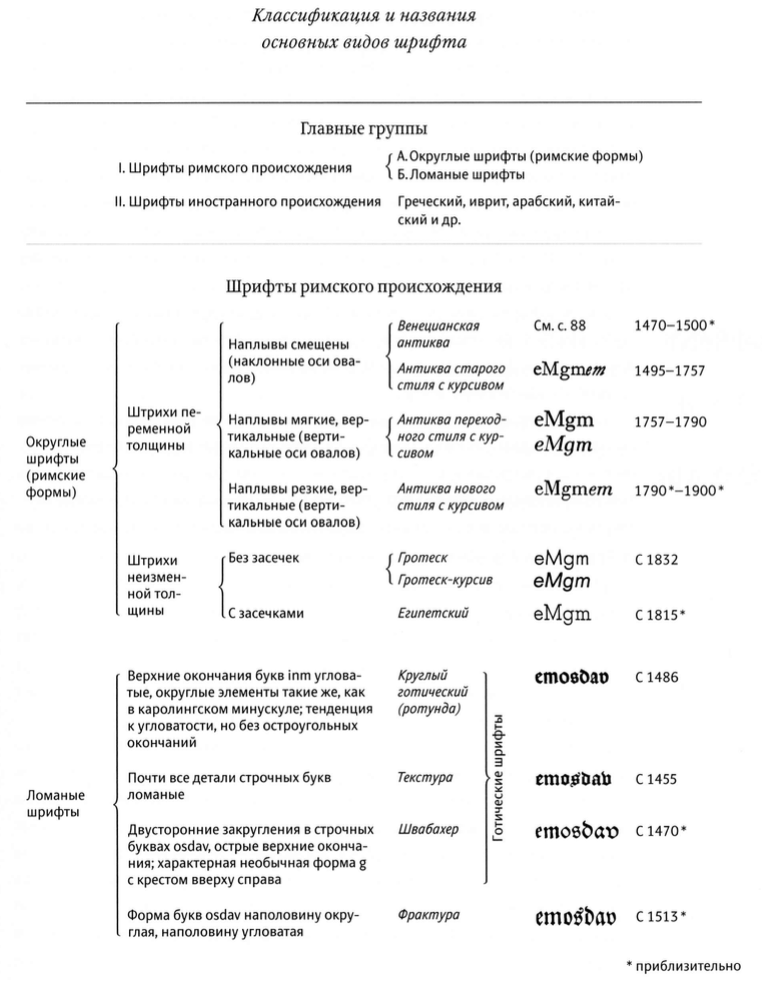
\includegraphics[width=\textwidth]{pics/fonts_class.png}
	\caption{Правило выбора полей книги}
	\label{fig:fonts_class}
\end{figure}

Также стоит отдельно упомянуть группу моноширинных гарнитур, в которых все глифы имеют одинаковую ширину. Например, в данном документе листинги набраны гарнитурой из такой категории --- Inconsolata.

Для большинства текстов рекомендуют выбирать кегль от 8pt до 14pt\footnote{хотя в разных гарнитурах размер глифов одного кегля могут быть отличными друг от друга}\cite{tschichold_aboutfont}.

У каждого элемента глифа существует свое название\cite{felichi_typo} (рисунок~\ref{fig:glyph_struct}).

\begin{figure}[H]
	\centering
	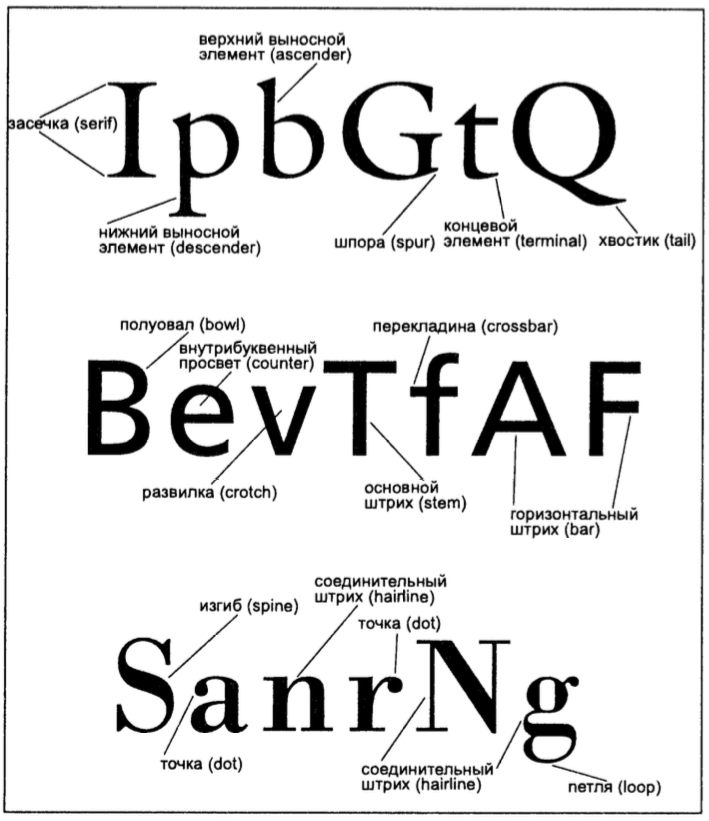
\includegraphics[width=0.55\textwidth]{pics/glyph_struct.png}
	\caption{Структура глифов}
	\label{fig:glyph_struct}
\end{figure}

При этом не в каждой гарнитуре присутствуют некоторые и элементов (например, засечки, петли и т.~п.)\cite{korolkova_livetypo}.